\documentclass[tikz,border=6pt]{standalone}
\begin{document}
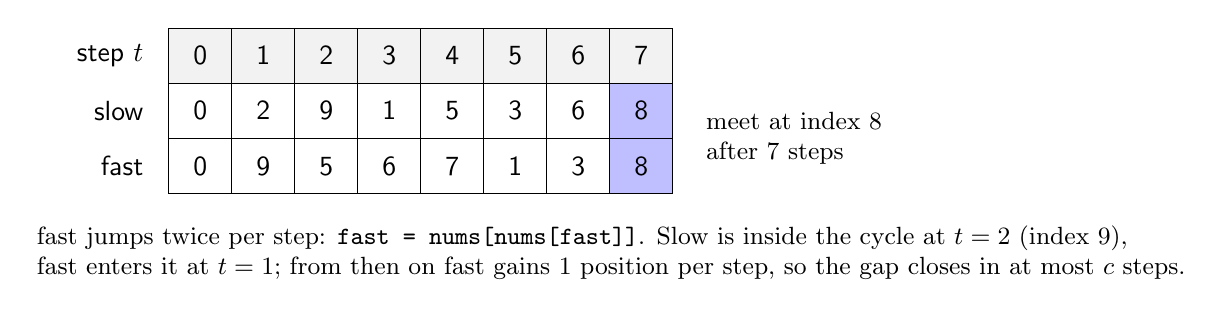
\begin{tikzpicture}[font=\sffamily,cell/.style={draw,minimum width=8mm,minimum height=7mm}]
\node[anchor=east] at (-0.6,0) {step $t$};
\node[anchor=east] at (-0.6,-0.7) {slow};
\node[anchor=east] at (-0.6,-1.4) {fast};
\def\slow{0,2,9,1,5,3,6,8}
\def\fast{0,9,5,6,7,1,3,8}
\foreach \s [count=\t from 0] in \slow { \node[cell,fill=gray!10] at (\t*0.8,0) {\t}; \node[cell] at (\t*0.8,-0.7) {\s}; }
\foreach \f [count=\t from 0] in \fast { \node[cell] at (\t*0.8,-1.4) {\f}; }
\node[cell,fill=blue!25] at (7*0.8,-0.7) {8}; \node[cell,fill=blue!25] at (7*0.8,-1.4) {8};
\node[anchor=west,font=\small,align=left] at (6.3,-1.05) {meet at index 8\\after 7 steps};
\node[anchor=west,font=\small,align=left] at (-2.2,-2.5) {fast jumps twice per step: \texttt{fast = nums[nums[fast]]}. Slow is inside the cycle at $t=2$ (index 9), \\fast enters it at $t=1$; from then on fast gains 1 position per step, so the gap closes in at most $c$ steps.};
\end{tikzpicture}
\end{document}
